\documentclass[a4paper,english]{article}
\usepackage{babel}
\usepackage[utf8]{inputenc}
\usepackage[T1]{fontenc}
\usepackage{times}
\usepackage[pdftex]{graphicx}
\usepackage{color}
\usepackage[pdftex,colorlinks=true,citecolor=black,
            pagecolor=black,linkcolor=black,menucolor=black,
            urlcolor=black]{hyperref}
\usepackage{epstopdf} % addition to include eps
\usepackage{eufrak}
\usepackage{amsmath}
\usepackage{amsbsy}
\usepackage{eucal}
%\usepackage{caption}
%\usepackage{subcaption} % for subfigures
\usepackage{subfig}
\usepackage{longtable}
\usepackage{url}
\urlstyle{same}
\usepackage{setspace}
\usepackage{natbib}
\usepackage{listings}
\usepackage{algorithm, algorithmic}
\usepackage[version=3]{mhchem} % for chemical reactions

\pdfinfo{            
          /Title      (T-61.5110 Modeling of Biological Networks)
          /Author     (Arttu Modig)
          /Keywords   ()          
}


\title{T-61.5110 Modeling of Biological Networks \\ Exercise Session 7}
\author{Arttu Modig \\ 79358S \\
       {\it arttu.modig@aalto.fi}}


\begin{document}
%--- KANSILEHTI -------------------------------------------------------------
\maketitle


%\newpage
%------------------------------------------------------------------------------
\onehalfspacing
\section{Bayesian network structure}
\subsection*{a}
The \texttt{blearn}-package contains algorithms and visualization tools for Bayesian network structure learning, parameter learning, and inference. It has constraint-based, score-based and hybrid learning algorithms, local discovery algorithms, Bayesian network classifiers, independence tests and networks scores etc.

\subsection*{b}
The \texttt{learning.test} data set contains synthetic test data which has 5000 samples from probability distributions (see \texttt{learning.test.R} how the set is created). A, B, C, D and E are three-level factors with levels a, b and c. F is a two-level factor with levels a and b. The correct network structure is ([A][C][F][B|A][D|A,C][E|B,F]).

Hill-climbing algorithm is a score-based greedy search on the space of the directed graphs. It's an iterative algorithm that attempts to find a better solution by incrementally changing single elements of the solution. It's good for finding a local optimum but not guaranteed to find the global optimum. Hill climbing differs from gradient descent methods which adjust all of the values of the solution at each iteration. The hill-climbing may have problems with spaces that have ridges, alleys and plateaus.

\begin{figure}[htp]
    \begin{center}
        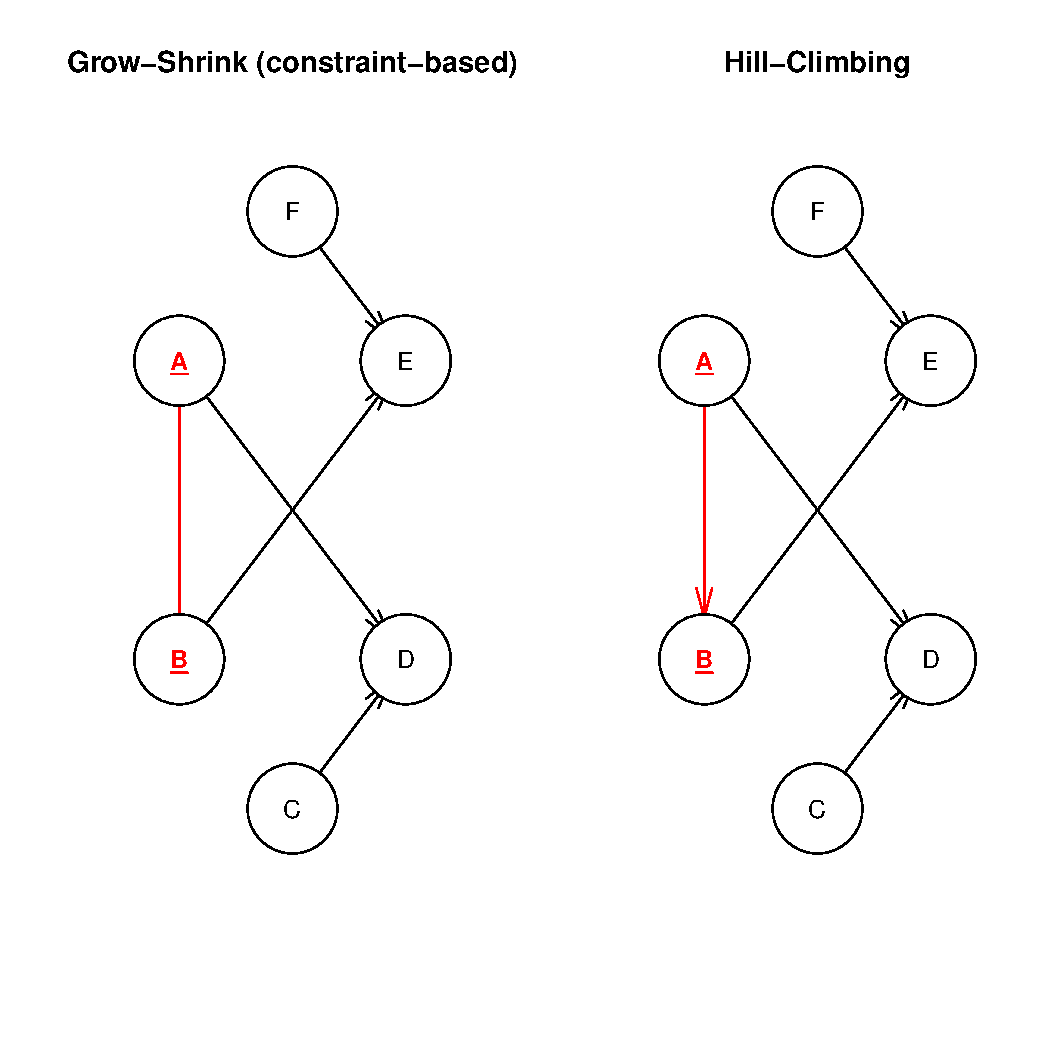
\includegraphics[width=0.66\textwidth]{graphs.pdf}
        \caption{The test graphs from two different structure learning methods.} \label{fig:graph}
    \end{center}
\end{figure}

\begin{figure}[htp]
    \begin{center}
        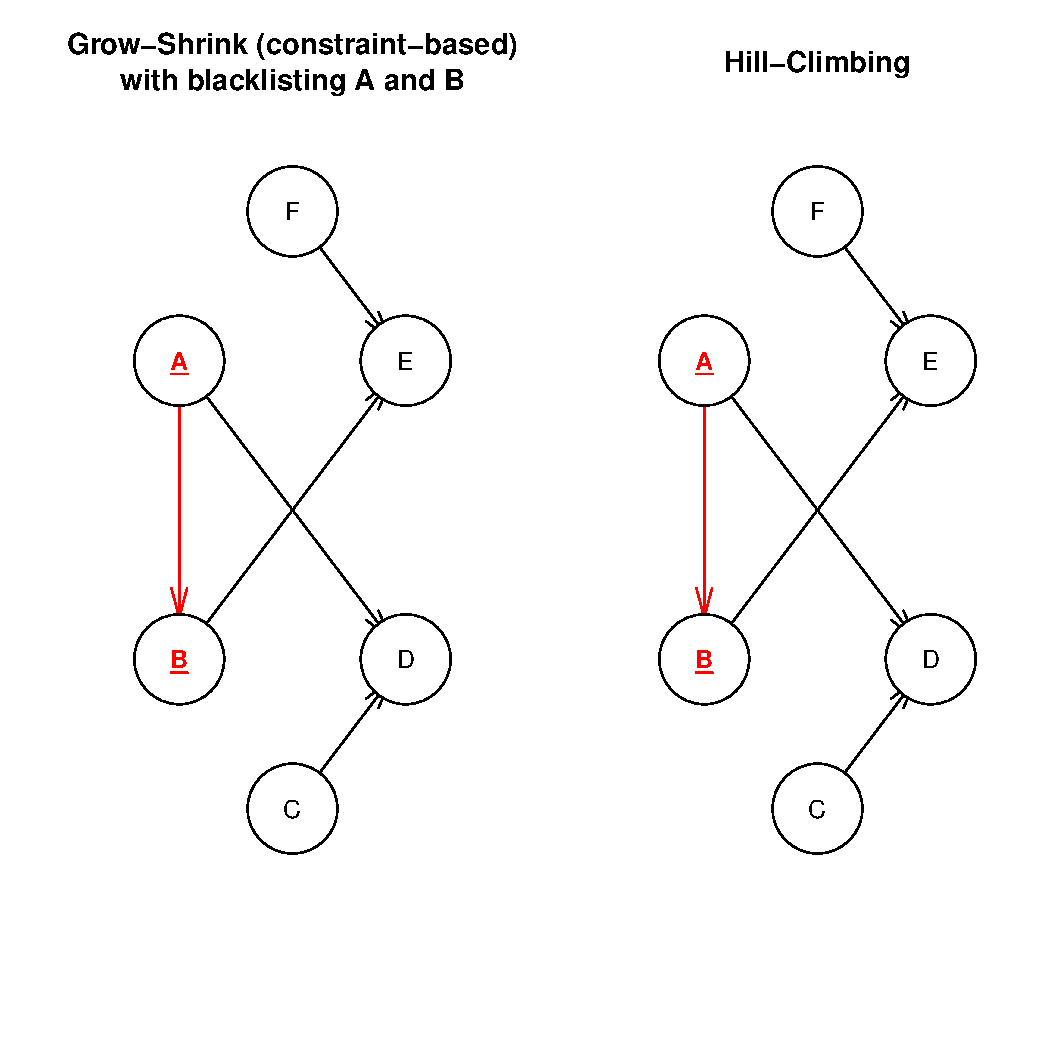
\includegraphics[width=0.66\textwidth]{graphs2.pdf}
        \caption{The test graphs from two different structure learning methods. Now arch B to A has been blacklisted in Grow-Shrink algorithm.} \label{fig:graph2}
    \end{center}
\end{figure}

\subsection*{c}
The Grow-Shrink algorithm is a structure learning algorithm based on the simplest Markov blanket detection algorithm called \emph{Grow-Shrink Markov Blanket}. The algorithm is explained e.g. in this paper: \url{http://jmlr.org/papers/volume9/pellet08a/pellet08a.pdf}.

As GS is constraint-based learning and it tries to find equivalence classes with Markoc blankets. With this test data set, it does not make a conditional distinction between factors A and B which can be seen in Figure \ref{fig:graph}. Also, the GS algorithm uses 43 test when hill-climbing uses 40.

\subsection*{d}
If however we use some expert knowledge for constraint-based learning (or from an other method such as hill-climbing), we can use this knowledge to re-train the model. Here with Grow-Shrink algorithm we blacklist the arc from B to A. This has the result that after training with GS algorithm the model has only the arc from A to B, so the resulting model is the same as with hill-climbing algorithm. See Figure \ref{fig:graph2}.

\section{More Bayesian networks}
As the dataset is continuous variables, we first discretize the data using \emph{Hartemink’s pairwise mutual information} method with 3 levels: LOW, AVG, HIGH. The directed network strengths are computed with hill-climbing algorithm, using two different methods: bootstrapping and creating random graphs. We generate 500 random networks with \emph{melancon} algorithm (with uniform probability over all possible graphs), and then we apply the hill-climbing to train the random networks. We use model averaging to build a network consisting of only significant arcs. Similar analysis is done with the bootstrapping algorithm.

The results show that the models have the same BDE-score (the logarithm of the \emph{Bayesian Dirichlet equivalent score}), and the models have the same \emph{moral graphs}, but the models have different arch sets. The bootstrapped average network is in Figure \ref{fig:boot} and the hill-climbed average netwok is in Figure \ref{fig:start}. The differences have been hilighted. We can see that the conditional relationship between factors PIP2 and PIP3 is different between the models.


\begin{figure}[htp]
    \begin{center}
        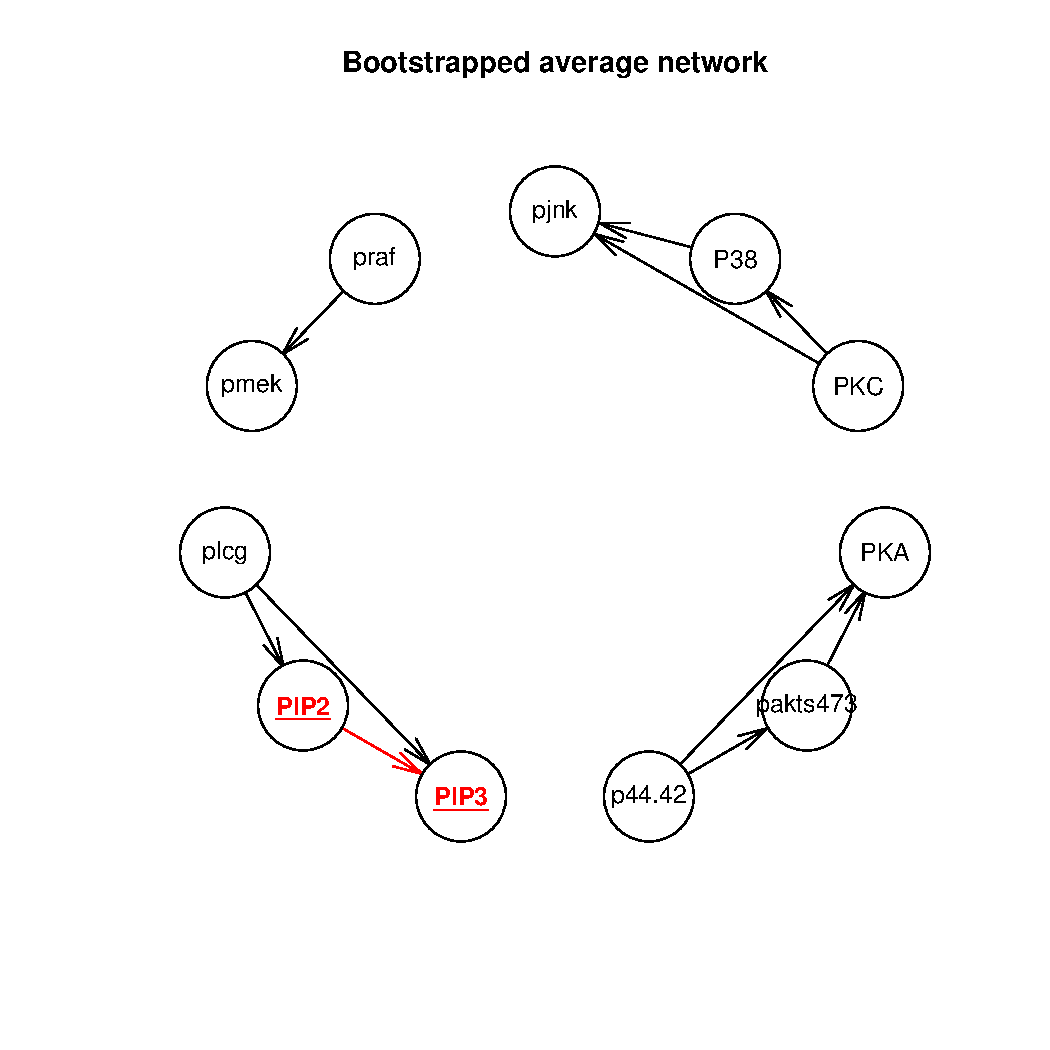
\includegraphics[width=0.66\textwidth]{boot.pdf}
        \caption{The average network by bootstrapping.}
        \label{fig:boot}
    \end{center}
\end{figure}

\begin{figure}[htp]
    \begin{center}
        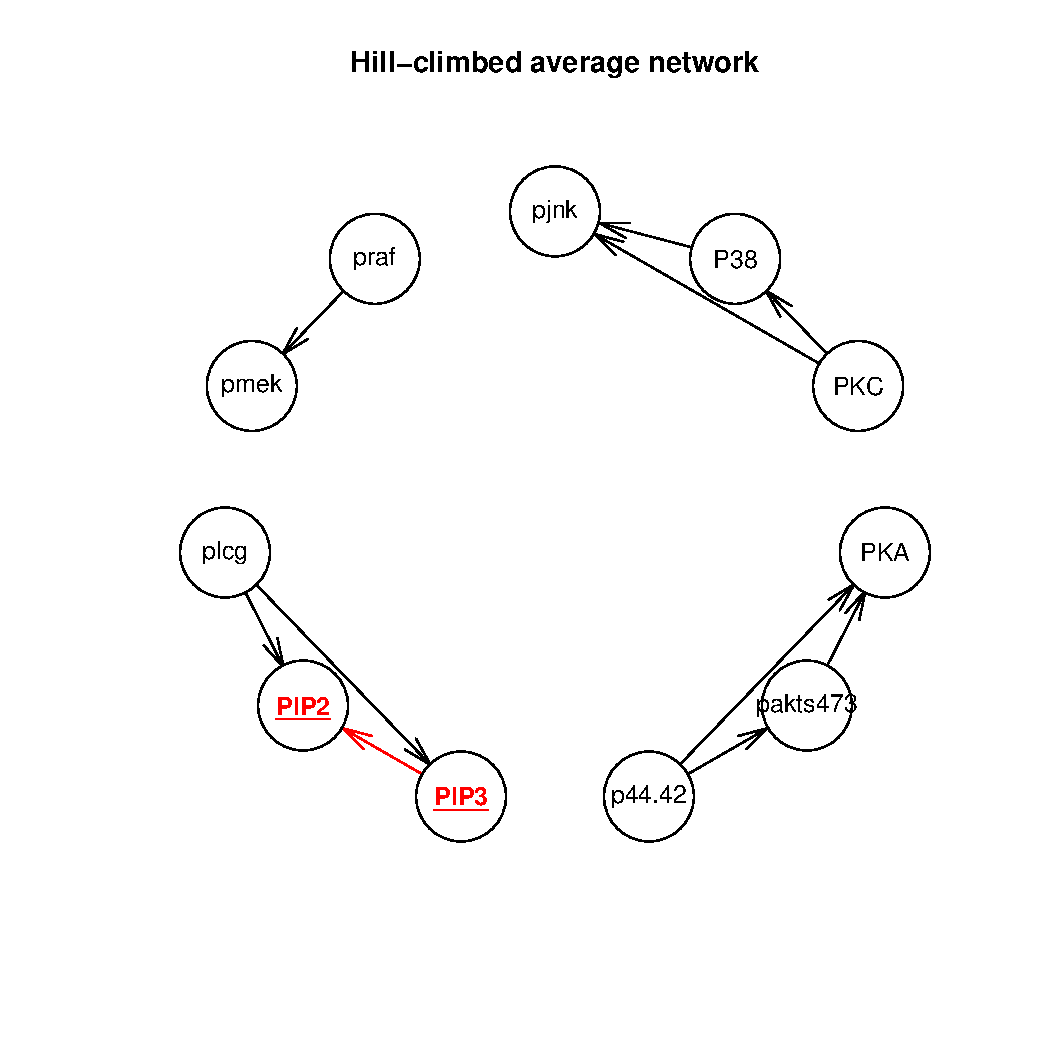
\includegraphics[width=0.66\textwidth]{start.pdf}
        \caption{The average network created by random graph sampling.}
        \label{fig:start}
    \end{center}
\end{figure}


\end{document}

%%% Local Variables: 
%%% mode: latex
%%% TeX-master: t
%%% End: 
